% $Id: Factories.tex,v 1.2 2008/10/09 16:16:11 dconway Exp $
\chapter{\label{chapter:Factories}Factories and Subscribers}
\chapauthor{Darrel J. Conway}{Thinking Systems, Inc.}

Chapter~\ref{chapter:Moderator} through \ref{chapter:Publisher} discussed the components of
GMAT's engine that are used to drive the flight dynamics model.  This chapter discusses two elements
used by the engine to construct and view the model during a run of the model: the Factory classes
and the Subscribers.

\section{\label{section:FactoryClasses}The Factory Classes}

The object factory components are responsible for creating instances of the classes registered with
GMAT for use in a run.  Each factory is configured as a node in a list.  The factory classes include
links to owned factories as well, allowing the creation of a tree structure for the factory system.

Each Factory maintains a list of core classes that it knows how to instantiate.  All of the core
classes are derived from a base class, GmatBase, which provides basic structure for
the created objects.  Each of the core objects has a group ID used to identify what type of object
it is, the name of the object's type (e.g. RungeKutta89, Drag, Spacecraft, Groundstation, etc), and
the instance's name.  The GmatBase class also provides a mechanism to find the parameter list for
instantiated objects, so that the list of available parameters can be built through calls to an
instance of a class that is being configured.

The Moderator builds lists of the recognized objects on request.  This feature allows a user
interface to make a call through the User Action Interpreter to get a list of the available objects
by class.  The Moderator can be asked for all of the objects configured in the system or all objects
of a specified type (e.g. Propagators).  This list can be used to populate selection lists in the
UI.  Once a user selects a specific type of object for configuration, the UI can make a call through
the Moderator to obtain an instance of the corresponding Atom.  That Atom is then instantiated, and
the UI makes calls to the created instance to get the list of available parameters, and to set the
values for each parameter.

The Moderator creates instances of each registered Factory during the initialization sequence.  GMAT
starts with a set of core factories that are always instantiated when the system starts.  Users can
create additional Factories and add them to GMAT dynamically.  User created factories are placed in
shared libraries compiled for the platform running GMAT -- for Windows, user created
Factories are built into DLLs; under Linux and OS X, they are built into shared libraries.

\subsection{Factory Attributes and Interfaces}

Each Factory fills in the table of creatable objects and implements code to call the constructors
for the creatable types.  The following lists describe the attributes and methods in the base class
that provide these functions.

\subparagraph{\textit{Class Attributes}}

The current factories are tailored to support a single core type in each factory, represented by
the itsType member.  All current factories are case sensitive as well.  The factory attribute list
is presented here:

\begin{itemize}
\item \textbf{Gmat::ObjectType itsType}: The type supported by the Factory.
\item \textbf{StringArray creatables}: The list of creatable objects.
\item \textbf{bool isCaseSensitive}: A flag indicating if the type name is case sensitive for the
factory.
\end{itemize}

\subparagraph{\textit{Methods}}

The Factory instances implement

\begin{itemize}
\item \textbf{virtual GmatBase* CreateObject(const std::string \&ofType, const std::string
\&withName = "")}:  Creates an object of the specified type with the specified name, and returns
the object as a GmatBase pointer.
\item \textbf{virtual SpaceObject* CreateSpacecraft(const std::string \&ofType, const std::string
\&withName = "")}:  Creates a SpaceObject object of the specified type with the specified
name, and returns the object as a SpaceObject pointer.
\item \textbf{virtual Propagator* CreatePropagator(const std::string \&ofType, const std::string
\&withName = "")}:  Creates a propagtor object of the specified type with the specified name, and
returns the object as a Propagator pointer.
\item \textbf{virtual ForceModel* CreateForceModel(const std::string \&ofType, const std::string
\&withName = "")}:  Creates a ForceModel object of the specified type with the specified name, and
returns the object as a ForceModel pointer.
\item \textbf{virtual PhysicalModel* CreatePhysicalModel(const std::string \&ofType, const
std::string \&withName = "")}:  Creates a Force used in a ForceModel of the specified type
with the specified name, and returns the object as a PhysicalModel pointer.
\item \textbf{virtual PropSetup* CreatePropSetup(const std::string \&ofType, const std::string
\&withName = "")}:  Creates a PropSetup object of the specified type with the specified name, and
returns the object as a PropSetup pointer.
\item \textbf{virtual Parameter* CreateParameter(const std::string \&ofType, const std::string
\&withName = "")}:  Creates a calculated parameter object of the specified type with the specified
name, and returns the object as a Parameter pointer.
\item \textbf{virtual Burn* CreateBurn(const std::string \&ofType, const std::string \&withName =
"")}:  Creates a burn object of the specified type with the specified name, and returns
the object as a Burn pointer.
\item \textbf{virtual StopCondition* CreateStopCondition(const std::string \&ofType, const
std::string \&withName = "")}:  Creates a stopping condition object of the specified type with the
specified name, and returns the object as a StopCondition pointer.
\item \textbf{virtual CalculatedPoint* CreateCalculatedPoint(const std::string \&ofType, const
std::string \&withName = "")}:  Creates a calculated point SpacePoint of the specified type with
the specified name, and returns the object as a CalculatedPoint pointer.
\item \textbf{virtual CelestialBody* CreateCelestialBody(const std::string \&ofType, const
std::string \&withName = "")}:  Creates a celestial body object of the specified type with the
specified name, and returns the object as a CelestialBody pointer.
\item \textbf{virtual SolarSystem* CreateSolarSystem(const std::string \&ofType, const std::string
\&withName = "")}:  Creates a SolarSystem object of the specified type with the specified name, and
returns the object as a SolarSystem pointer.
\item \textbf{virtual Solver* CreateSolver(const std::string \&ofType, const std::string \&withName
= "")}:  Creates a Solver object of the specified type with the specified name, and returns
the object as a Solver pointer.
\item \textbf{virtual Subscriber* CreateSubscriber(const std::string \&ofType, const std::string
\&withName = "", const std::string \&fileName = "")}:  Creates a subscriber object of the specified
type with the specified name, and returns the object as a Subscriber pointer.
\item \textbf{virtual GmatCommand* CreateCommand(const std::string \&ofType, const std::string
\&withName = "")}:  Creates a Command for use in the Mission Control Sequence of the specified type
with the specified name, and returns the object as a GmatCommand pointer.
\item \textbf{virtual AtmosphereModel* CreateAtmosphereModel(const std::string \&ofType, const
std::string \&withName = "", const std::string \&forBody = "Earth")}:  Creates an atmosphere model
of the specified type with the specified name, and returns the object as a AtmosphereModel pointer.
\item \textbf{virtual Function* CreateFunction(const std::string \&ofType, const std::string
\&withName = "")}:  Creates a user defined function of the specified type with the specified name,
and returns the object as a Function pointer.
\item \textbf{virtual Hardware* CreateHardware(const std::string \&ofType, const std::string
\&withName = "")}:  Creates a hardware object of the specified type with the specified name, and
returns the object as a Hardware pointer.
\item \textbf{virtual AxisSystem* CreateAxisSystem(const std::string \&ofType, const std::string
\&withName = "")}:  Creates an axis system as used in the coordimate system classes, of the
specified type with the specified name, and returns the object as an AxisSystem pointer.
\item \textbf{virtual CoordinateSystem* CreateCoordinateSystem(const std::string \&ofType, const
std::string \&withName = "")}:  Creates a coordinate system object of the specified type with the
specified name, and returns the object as a CoordinateSystem pointer.
\item \textbf{virtual MathNode* CreateMathNode(const std::string \&ofType, const std::string
\&withName = "")}:  Creates a node for use in a mathematical expression, of the specified type with
the specified name, and returns the object as a MathNode pointer.
\item \textbf{virtual Attitude* CreateAttitude(const std::string \&ofType, const std::string
\&withName = "")}:  Creates an attitude object of the specified type with the specified name, and
returns the object as a Attitude pointer.
\item \textbf{StringArray GetListOfCreatableObjects() const}: Returns the list of object types that
can be created by this Factory.
\item \textbf{bool SetListOfCreatableObjects(StringArray newList)}: Resets the list of creatable
objects.
\item \textbf{bool AddCreatableObjects(StringArray newList)}: Extends the list of creatable
objects.
\item \textbf{Gmat::ObjectType GetFactoryType() const}: Returns the type of the factory.
\item \textbf{bool IsTypeCaseSensitive() const}: Returns true if the creatable object type names
are case sensitive, false otherwise.
\end{itemize}

\subsection{An example: The BurnFactory}

Listing~\ref{listing:BurnFactory} shows the complete code implementing the BurnFactory
class\footnote{Comments and extra space have been removed from this listing to make it as short as
possible.}.  At this writing, GMAT supports two Burn classes, named ImpulsiveBurn and FiniteBurn.
The CreateBurn() method is used to build instances of these classes, as can be seen on
lines~\ref{line:BurnCreationStart} through~\ref{line:BurnCreationEnd}.  Each of the constructors for
the Factory needs to register the types of objects that can be created.  This registration of
accomplished by adding the string describing the supported object to the creatables StringArray
attrinute.  An example of this is shown on lines~\ref{line:CreatableFillingStart}
through~\ref{line:CreatableFillingEnd}.\\

\lstset{numbers=left,firstnumber=1,escapeinside={(*@}{@*)}}
\begin{lstlisting}[caption={Complete Implementation of the BurnFactory},
label={listing:BurnFactory}]
#include "BurnFactory.hpp"
#include "ImpulsiveBurn.hpp"
#include "FiniteBurn.hpp"

(*@\label{line:BurnCreationStart}@*)// Creation method
Burn* BurnFactory::CreateBurn(const std::string &ofType,
                              const std::string &withName)
{
   if (ofType == "ImpulsiveBurn")
      return new ImpulsiveBurn(withName);
   else if (ofType == "FiniteBurn")
      return new FiniteBurn(withName);

   return NULL;   // doesn't match any known type of burn
(*@\label{line:BurnCreationEnd}@*)}


// Default constructor
BurnFactory::BurnFactory() :
   Factory     (Gmat::BURN)
{
(*@\label{line:CreatableFillingStart}@*)   if (creatables.empty())
   {
      creatables.push_back("ImpulsiveBurn");
      creatables.push_back("FiniteBurn");
(*@\label{line:CreatableFillingEnd}@*)   }
}

// Support for secondary base class constructor
BurnFactory::BurnFactory(StringArray createList) :
   Factory     (createList, Gmat::BURN)
{
}

// Copy constructor
BurnFactory::BurnFactory(const BurnFactory &fact) :
    Factory     (fact)
{
   if (creatables.empty())
   {
      creatables.push_back("ImpulsiveBurn");
      creatables.push_back("FiniteBurn");
   }
}

// Assignment operator for the BurnFactory base class.
BurnFactory& BurnFactory::operator=(const BurnFactory &fact)
{
   Factory::operator=(fact);
   return *this;
}

// Destructor for the BurnFactory class.
BurnFactory::~BurnFactory()
{
}
\end{lstlisting}
\lstset{numbers=none}

\subsection{\label{section:TwentyOneFactories}Twenty-One Factories}

\begin{figure}[htb]
\begin{center}
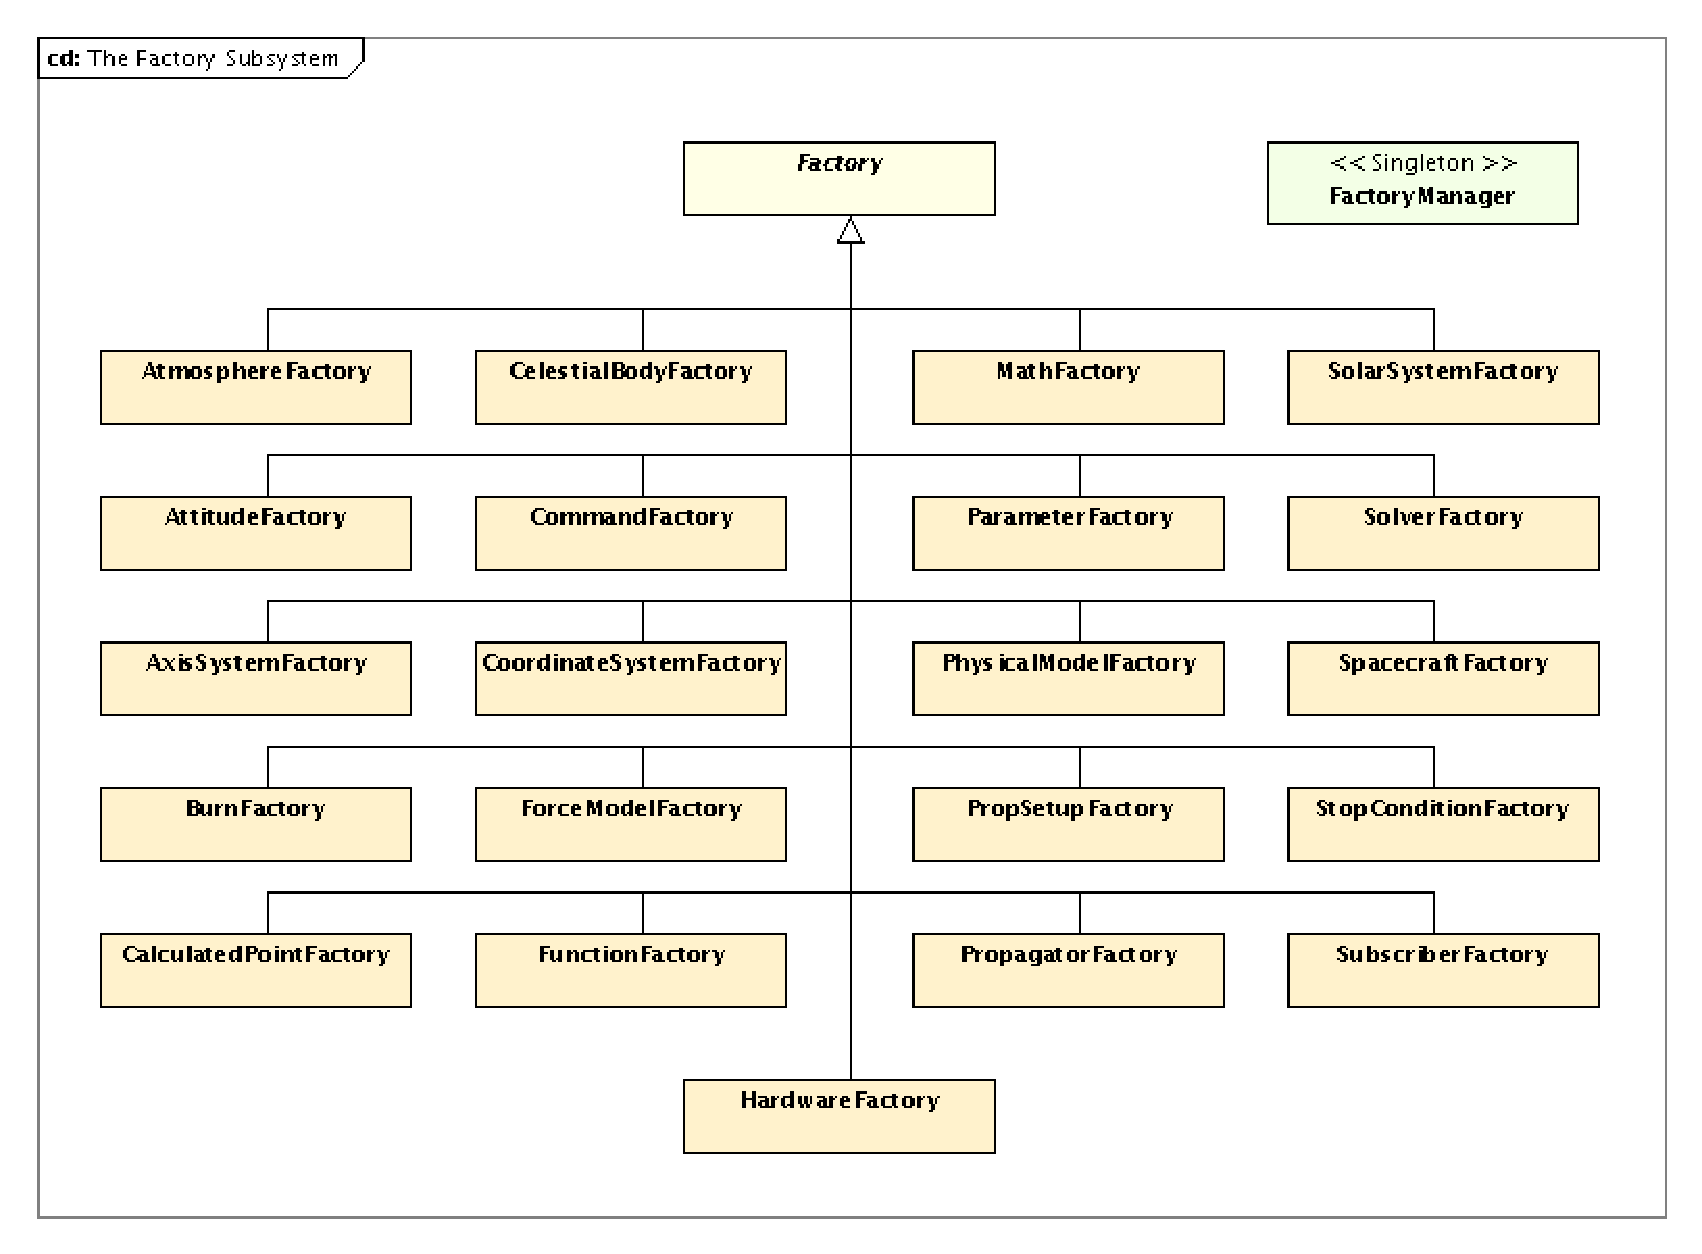
\includegraphics[scale=0.5]{Images/TheFactorySubsystem.eps}
\caption{\label{figure:TheFactorySubsystem}Class Hierarchy for 21 GMAT Factories}
\end{center}
\end{figure}

GMAT contains twenty-one factories at this writing, all implemented in a similar manner to that
shown in the previous section.  These factories are shown in
Figure~\ref{figure:TheFactorySubsystem}.

\subsection{\label{section:UserObjects}Extending GMAT}

Factories are a key element of GMAT's extensibility strategy.  A developer adds a new user component
to GMAT by taking the following steps:

\begin{enumerate}
  \item Design the new component based on GMAT's architecture.
  \item Code the new component, using GmatBase or one of its derivatives as the base class for the
component.
  \item Compile and debug the component as a stand-alone object (as much as possible).
  \item Create a new Factory that creates instances of the new component, or add the component to an
existing Factory\footnote{Factories can support many classes at once; if a convenient Factory
already exists for the developer, the new class can be added to that Factory without any loss of
functionality}.
  \item \label{item:RuntimeRegister}Either build a new shared library that contains the Factory and
the class or classes defining the new component, or incorporate the new classes and Factory in a
GMAT build.
  \item Register the new Factory with the Factory Manager.
  \item Test the new component in GMAT.
  \item Start using the new component.
\end{enumerate}

Note that step~\ref{item:RuntimeRegister} lists two possible ways to build the new code.
Chapter~\ref{chapter:ExtendingGMAT} provides a more thorough introduction to adding new classes to
GMAT, and includes a discussion of registering new components either at runtime or linked in at
compile time.

\begin{figure}[htb]
\begin{center}
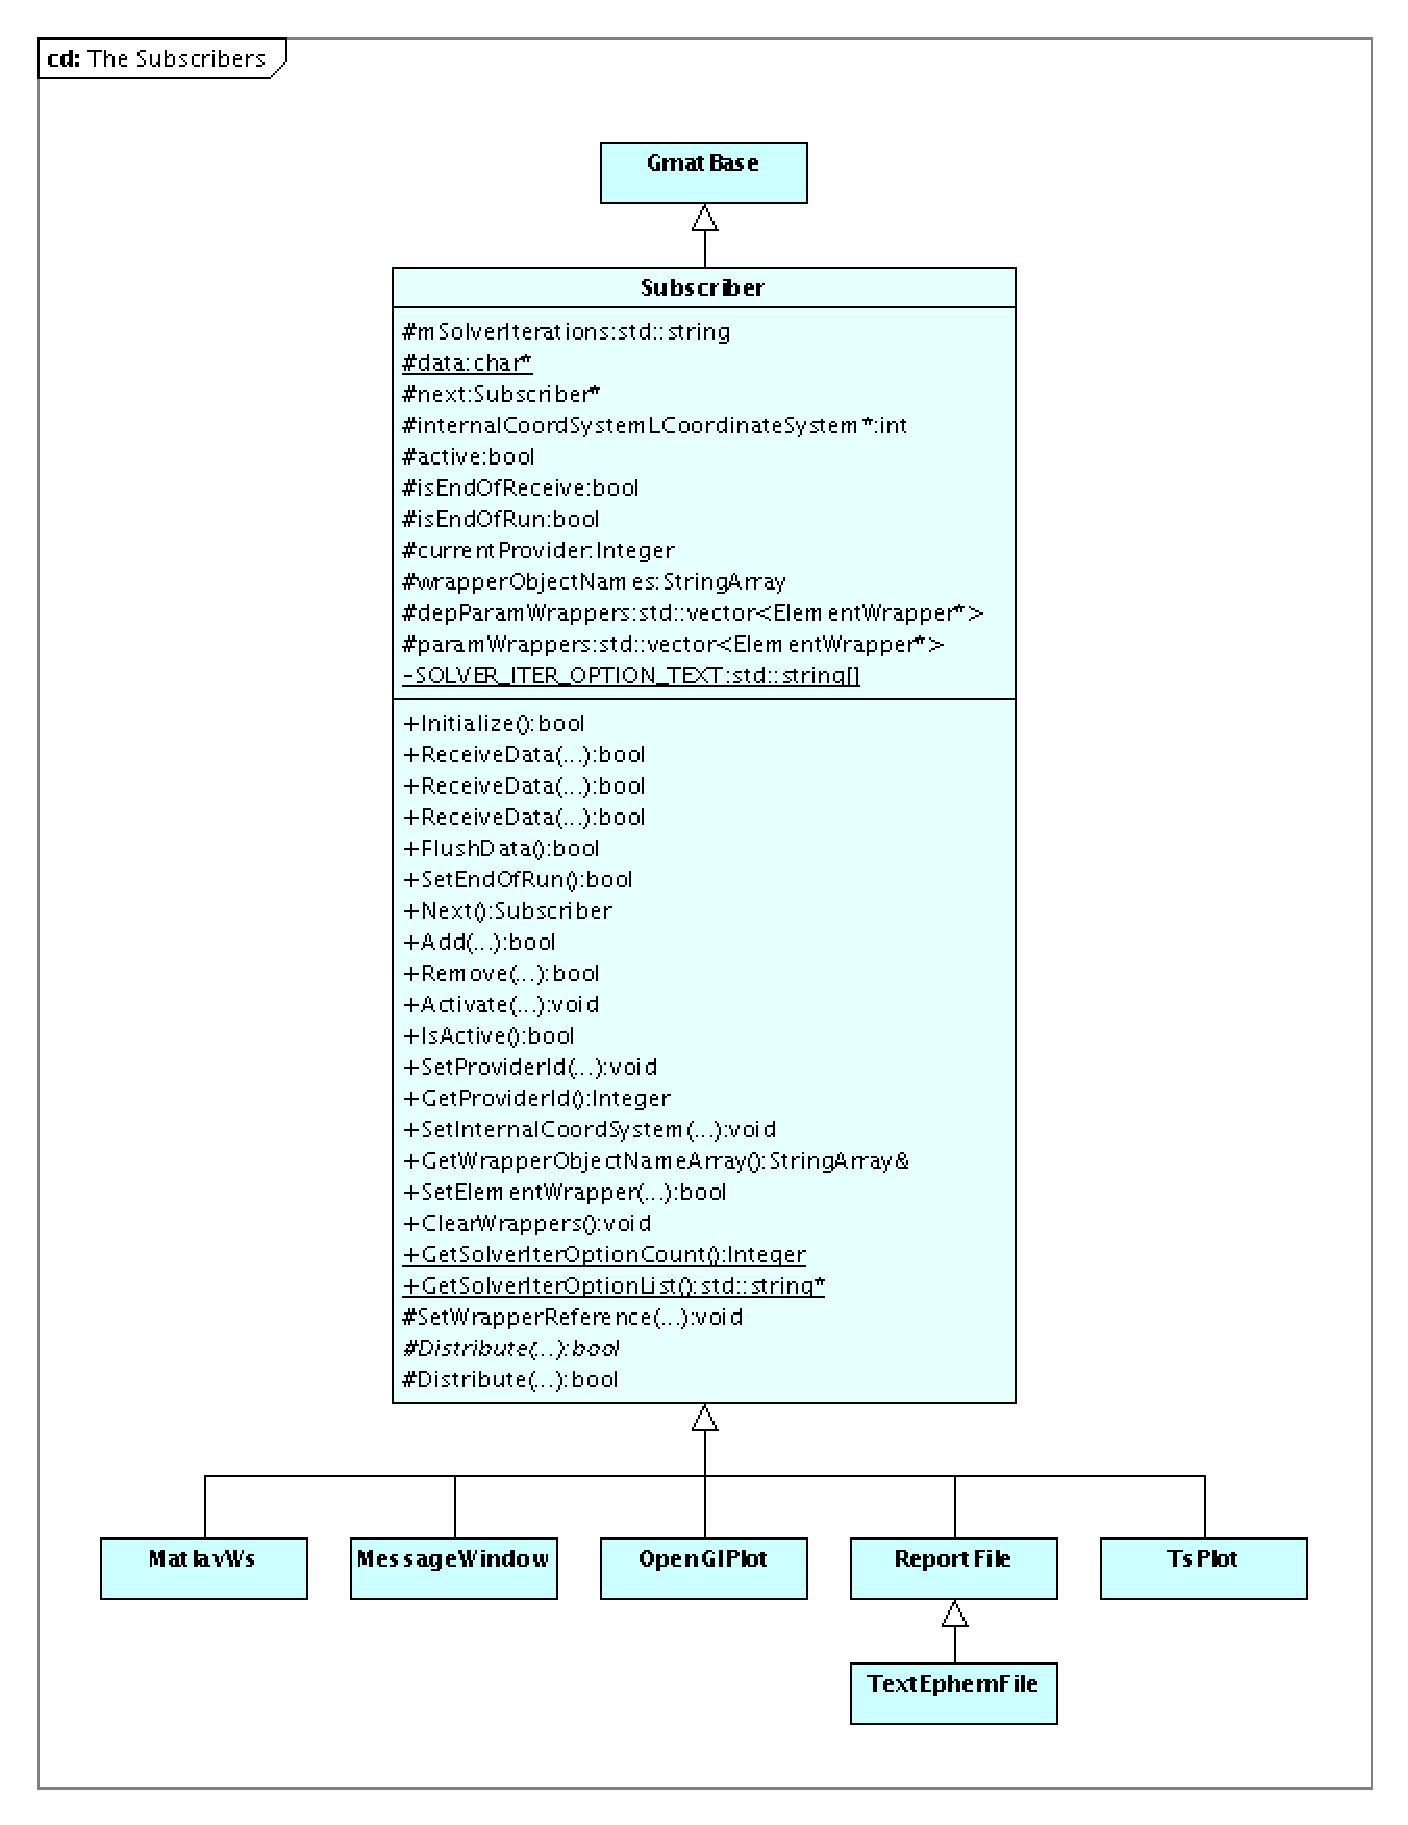
\includegraphics[scale=0.5]{Images/TheSubscribers.eps}
\caption{\label{figure:TheSubscribers}The Subscriber Class}
\end{center}
\end{figure}

\section{Subscribers}

During a Mission Control Sequence run data is sent from the Sandbox to GMAT's Publisher.  The
Publisher routes this data to two and three dimensional plots on the user's display, to report
files, and to any other output objects configured by the user prior to the run.  These output
objects are instances of classes derived from the Subscriber base class, shown in
Figure~\ref{figure:TheSubscribers}.

\subsection{Structure of the Subscribers}

The Subscribers all implement methods and structures designed to work as recipients of the data
delivered from GMAT's Publisher.  These members include several flags used to track the state of a
Mission Control Sequence run, wrappers used for published data, and methods used to pass the data
into the Subscribers and manage Subscriber processing.  The class members are describewd below.

\subparagraph{\textit{Class Attributes}}

\begin{itemize}
\item \textbf{std::string mSolverIterations}: Sets the behavior of the Subscriber when a Solver is
finding a solution.  The current options are ``All'' and ``None''.
\item \textbf{const char *data}: A pointer used in the ReceiveData method to set the input buffer
that is processed.
\item \textbf{CoordinateSystem *internalCoordSystem}: A coordinate system available for conversions
when needed.
\item \textbf{bool active}: Flag specifying if the Subscriber is currently processing data.
\item \textbf{bool isEndOfReceive}: Flag indicating that the current set of data has finished being
sent.
\item \textbf{bool isEndOfRun}: Flag indicating that the current Mission Control Sequence has
finished running.
\item \textbf{Gmat::RunState runstate}: The current run state of the Mission Control Sequence.
\item \textbf{Integer currentProvider}: The ID of the current data privider.
\item \textbf{StringArray wrapperObjectNames}: The list of data wrappers used by the Subscriber.
\item \textbf{std::vector<ElementWrapper*> depParamWrappers}: The data wrappers used for dependent
parameters.
\item \textbf{std::vector<ElementWrapper*> paramWrappers}: The data wrappers used for parameters.
\end{itemize}

\subparagraph{\textit{Methods}}

\begin{itemize}
\item \textbf{virtual bool Initialize()}:  Sets all internal pointers needed to use the Subscriber.
\item \textbf{virtual bool ReceiveData(const char* datastream)}: Receives character data from the
Publisher.  The data passed in is a standard C/C++ string, terminated with a NULL ('\\0')
character.
\item \textbf{virtual bool ReceiveData(const char* datastream, const Integer len)}: Receives
character data from the Publisher.  The data passed in fills a buffer of the indicated length.
\item \textbf{virtual bool ReceiveData(const Real* datastream, const Integer len = 0)}: Receives
Real number data from the Publisher.  The data passed inis in a C/C++ array of the indicated length.
\item \textbf{virtual bool FlushData()}: Method called to tell the Subscriber to process all
received data immediately.
\item \textbf{virtual bool SetEndOfRun()}: Tells the Subscriber that a Mission Control Sequence run
has been complted, so the Subscriber should process all unprocessed data.
\item \textbf{virtual bool SetRunState(Gmat::RunState rs)}: Updates the run state so the subscriber
can act based in state changes.
\item \textbf{void Activate(bool state = true)}: Changes the active flag to the input setting.
Subscribers can use this setting to toggle on or off the processing on input data.
\item \textbf{bool IsActive()}: Returns the value of the active flag.
\item \textbf{virtual void SetProviderId(Integer id)}:
\item \textbf{virtual Integer GetProviderId()}:
\item \textbf{virtual void SetInternalCoordSystem(CoordinateSystem *cs)}:
\item \textbf{virtual const StringArray\& GetWrapperObjectNameArray()}:
\item \textbf{virtual bool SetElementWrapper(ElementWrapper* toWrapper, const std::string \&name)}:
\item \textbf{virtual void ClearWrappers()}: Deletes and sets all wrapper pointers to NULL but
leaves size unchanged.
\item \textbf{static Integer GetSolverIterOptionCount()}:
\item \textbf{static const std::string* GetSolverIterOptionList()}:
\item \textbf{bool SetWrapperReference(GmatBase *obj, const std::string \&name)}:
\item \textbf{virtual bool Distribute(Integer len) = 0}:
\item \textbf{virtual bool Distribute(const Real *dat, Integer len)}:
\end{itemize}

\subparagraph{\textit{Deprecated Attributes and Methods}}

Subscribers were initially prototyped in a linked list structure.  Some artifacts of that design
remain in the current code, but will be removed in a later release.  These pieces are listed below.

\begin{itemize}
\item \textbf{Subscriber *next}: The pointer to the next Subscriber in the list.
\item \textbf{Subscriber* Next()}: Retrieves the next Subscriber for the current list.
\item \textbf{bool Add(Subscriber *s)}: Adds a Subscriber at the end of the list.
\item \textbf{bool Remove(Subscriber *s, const bool del)}: Removes a Subscriber from the list.
\end{itemize}

\subsection{Subscriber Initialization and Execution}

\subsubsection{Defining and Initializing Subscribers}

Each Subscriber in GMAT has an associated GmatBase derived object that is stored in the
configuration and cloned into the Sandbox prior to a run.  These objects are the connection points
between operations occuring in the Sandbox and the data presented to the user, either graphically
or in text form.

\subsubsection{Subscriber Usage During Mission Execution}

